\section{Tools and servers}\label{Tools-and-Servers}

The vitess tools and servers are designed to help you even
if you start small, and scale all the way to a complete fleet
of databases.

In the early stages, connection pooling, rowcache and other
efficiency features of vttablet help you get more from your
existing hardware.
As things scale out, the automation tools start to become handy.

\subsubsection{vtctl}\hypertarget{vtctl}{}\label{vtctl}

vtctl is the main tool for performing administrative operations.
It can be used to track shards, replication graphs and
db categories.
It's also used to initiate failovers, reshard, etc.

As vtctl performs operations, it updates the necessary
changes to the lockserver (zookeeper).
The rest of the vitess servers observe those changes
and react accordingly.
For example, if a master database if failed over to a new
one, the vitess servers will see the change and redirect
future writes to the new master.

\subsubsection{vttablet}\hypertarget{vttablet}{}\label{vttablet}

One of vttablet's main function is to be a proxy to MySQL.
It performs tasks that attempt to maximize throughput as
well as to protect MySQL from harmful queries. There is
one vttablet per MySQL instance.

vttablet is also capable of executing necessary management
tasks initiated from vtctl.
It also provides streaming services that are used for
filtered replication and data export.

\subsubsection{vtocc}\hypertarget{vtocc}{}\label{vtocc}

Vtocc is the previous version of vttablet. It handles query management
(same as vttablet) but is not part of a larger system, it's a standalone
program that doesn't require a Topology Server. It is useful for
unit tests and when the only required feature is the query service
(with connection pooling, query de-dup, ...).

Note we may eventually produce a version of vttablet that runs
without a Topology Server, and use it instead of vtocc.

\subsubsection{vtgate}\hypertarget{vtgate}{}\label{vtgate}

vtgate's goal is to provide a unified view of the entire fleet.
It will be the server that applications will connect to for
queries. It will analyze, rewrite and route queries to various
vttablets, and return the consolidated results back to the client.

\subsubsection{vtctld}\hypertarget{vtctld}{}\label{vtctld}

vtctld is an HTTP server that lets you browse the information stored
in the lockserver.
This is useful for trouble-shooting, or to get a good high
level picture of all the servers and their current state.

\subsubsection{vtworker}\hypertarget{vtworker}{}\label{vtworker}

vtworker is meant to host long-running processes. It supports a plugin infrastructure, and offers libraries to easily pick tablets to use. We have developped:
- resharding differ jobs: meant to check data integrity during shard splits and joins.
- vertical split differ jobs: meant to check data integrity during vertical splits and joins.

It is very easy to add other checker processes for in-tablet integrity checks (verifying foreign key-like relationships), and cross shard data integrity (for instance, if a keyspace contains an index table referencing data in another keyspace).

\subsubsection{vtprimecache}\hypertarget{vtprimecache}{}\label{vtprimecache}

vtprimecache is a mysql cache primer for faster replication. If the single MySQL replication thread is falling behind, vtprimecache activates and starts reading the available relay logs. It then uses a few threads / connections to MySQL to execute modified statements and prime the MySQL buffer cache. The idea is for instance if an 'update table X where id=2' statement is going to be executed by the replication SQL thread 2 or 3 seconds from now, might as well execute a concurrent 'select from table X where id=2' now and prime the MySQL buffer cache. In practice, this shows a speed improvement in replication speed by 30 to 40 percents.

\subsubsection{Other support tools}\hypertarget{other-support-tools}{}\label{other-support-tools}

\begin{itemize}
\item \emph{mysqlctl}: manage MySQL instances.
\item \emph{zkctl}: manage ZooKeeper instances.
\item \emph{zk}: command line ZooKeeper client and explorer.
\end{itemize}

\subsection{Vitess components block diagram}\hypertarget{vitess-components-block-diagram}{}\label{vitess-components-block-diagram}

\begin{figure}[H]
\caption{components block diagram}
\label{fig:Vitess Spectrum}
\begin{center}
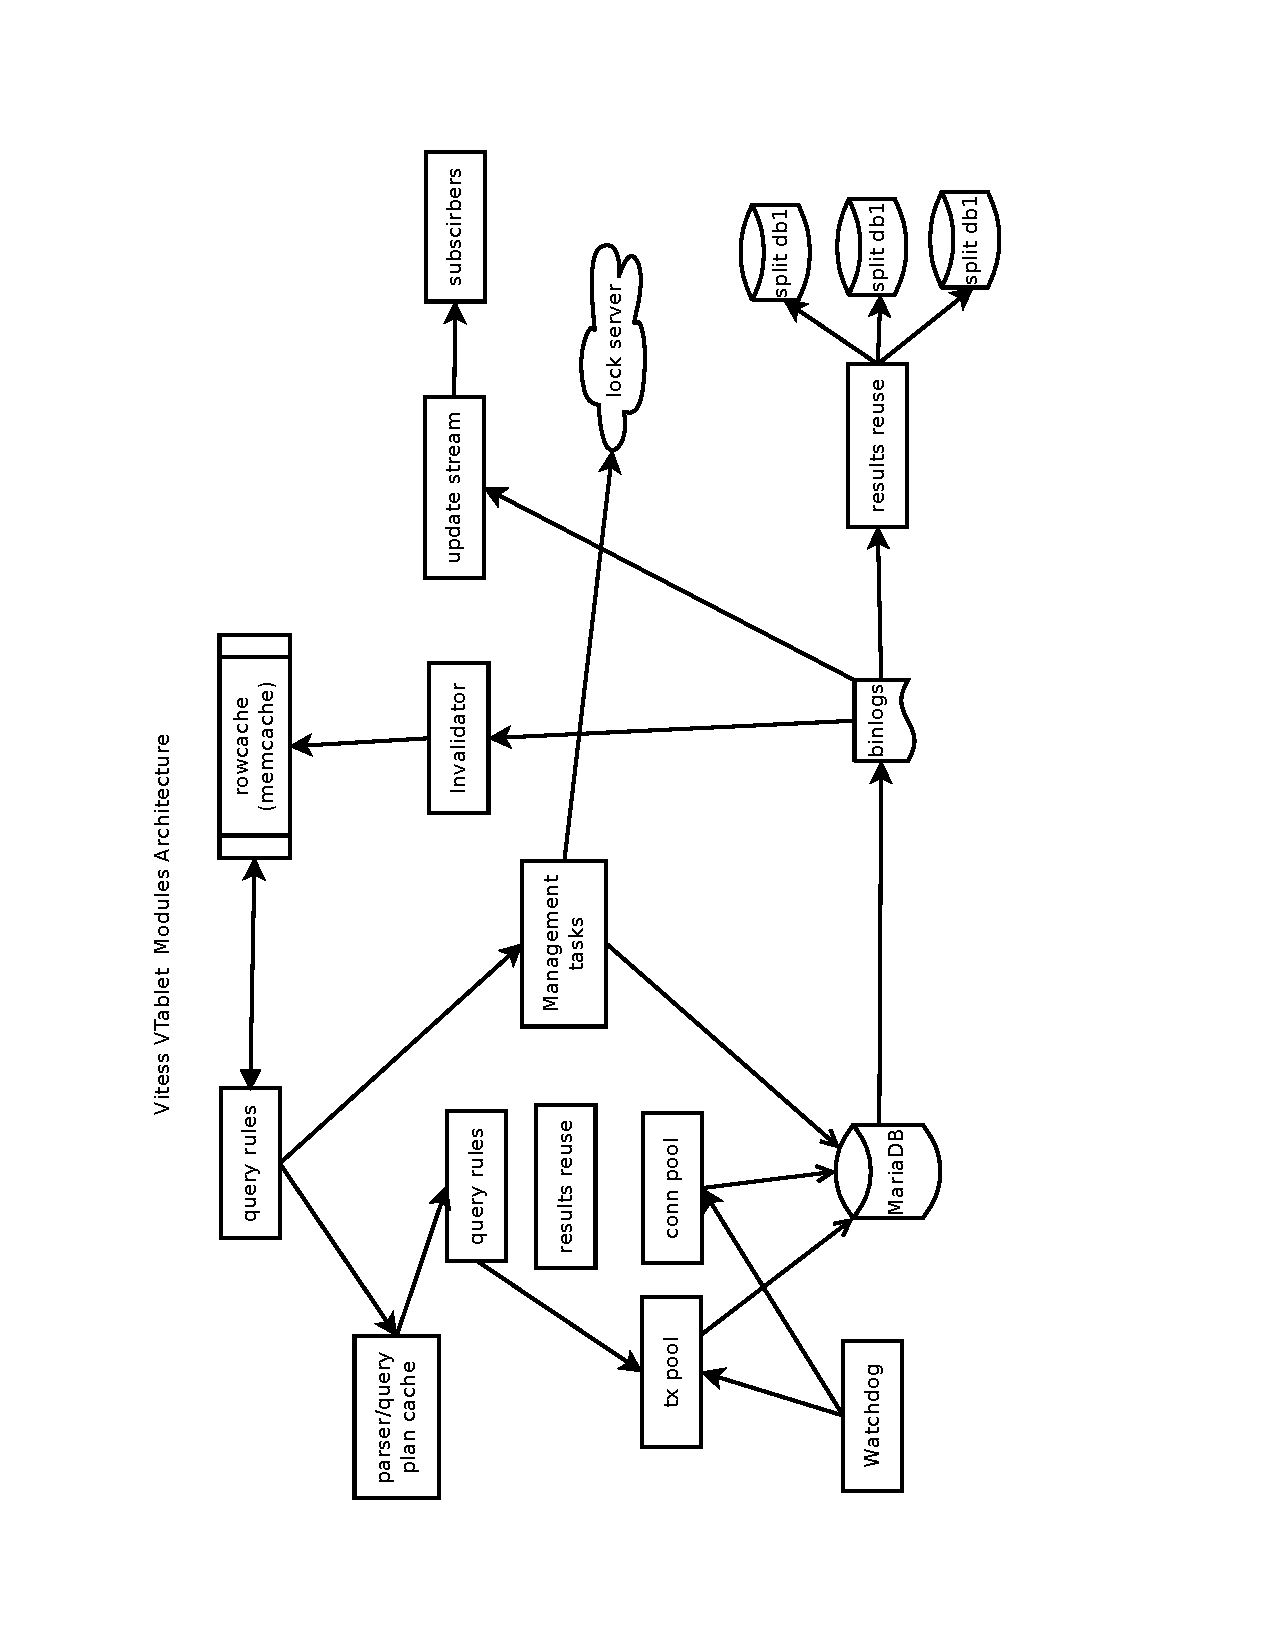
\includegraphics[scale=0.65]{VTTabletModules.pdf}
\end{center}
\end{figure}





